\chapter{Introduction}

In the Netflix animated series Cyberpunk: Edgerunners \parencite{cyberpunk_2022}, the main character attends courses at a 
prestigious academy that uses advanced technology to boost education and performance. The students gather in a room with
Virtual Reality \ac{VR} headsets and connect to the lesson, which is taught by a holographic (and probably powered by artificial
intelligence) tutor. The episode does not show the lesson itself (the entire system fails catastrophically when attacked by
malware), but the brief scene highlights the vision many people have of a futuristic classroom, one guided by advanced technology
and automatization.

\begin{figure}[t]
    \centering{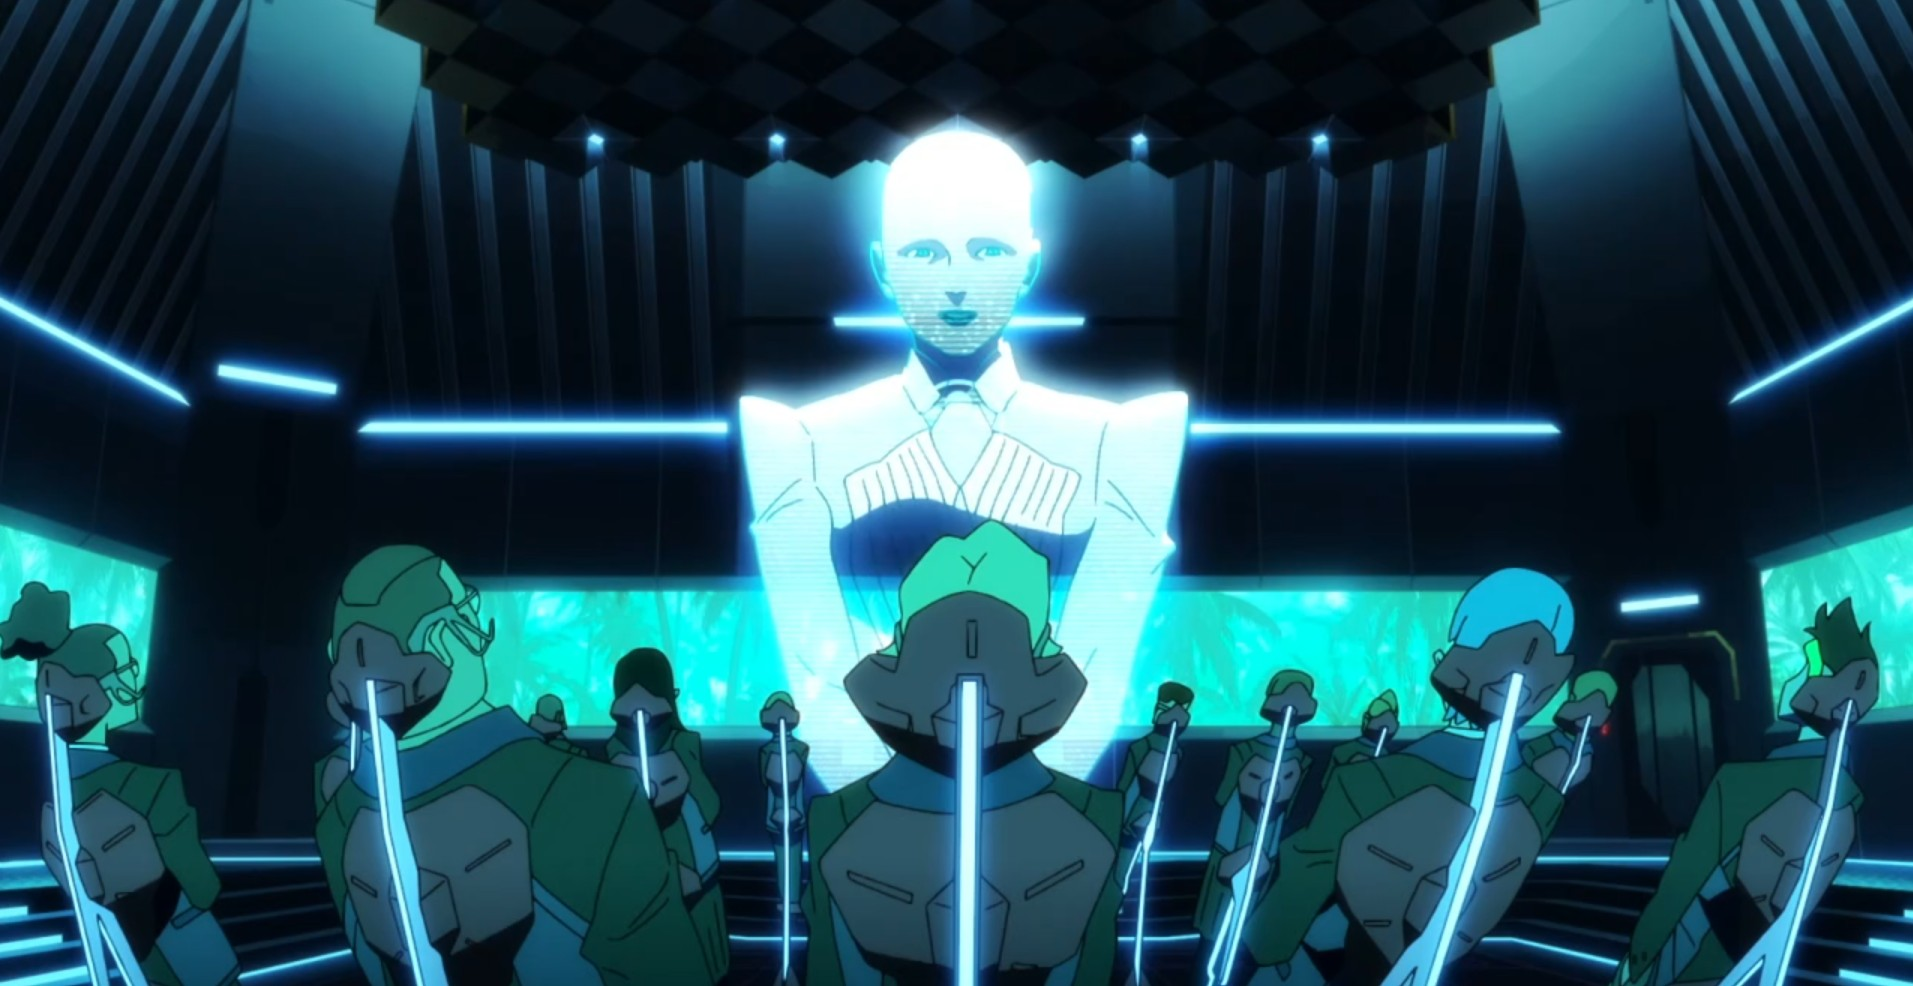
\includegraphics[alt={Figure 1.1},width=0.99\textwidth]{figures/F1-1.jpg}}
    \caption{Virtual Classroom in Cyberpunk: Edgerunners\label{fig:1-1}}
\end{figure}

\textcite{forsler_2024} propose the term “post-digital classroom” to identify the characteristics and trends in education
present in a world beyond the adoption of digital technologies. The purpose of this classroom is not anymore to
introduce new technologies to students, but to implement them as an essential factor of the learning process. The
post-digital classroom is interconnected, social and global. In this scenario, learning goes beyond the physical
classroom because it is based on creating relationships between concepts and developing valuable skills rather than
acquiring knowledge. It is also a classroom where information is detached from the physical learning institute, and
access to facts and sources is, ideally, immediate, ubiquitous and democratic.

The classroom has also become hybrid. There is little distinction between network-based lessons and the face-to-face spaces
associated with schools and universities \parencite{goodyear_2004}. Hybrid and blended approaches blur the distinctions
between learning in an online setting and learning in a classroom. In both instances, information is at hand in the network,
students can easily connect to peers and mentors, distance and time constrains are less meaningful and knowledge is presented
in a multimedia format that needs a technological backbone to be created and shared \parencite{rivoltella_2008,shank_2005}.

This thesis explores the use of technology in such post-digital classrooms, specifically, Augmented Reality \ac{AR} within the
context of mobile computing. Moreover, this research will analyse the creation of effective learning spaces, those places where
students can build, personalise and control all the activities they engage with \parencite{gourlay_2016}. Learning spaces are
interesting tools at the disposal of students because these are spaces that can exist outside the norm of a typical classroom,
they are more fluid, less structured and can easily connect to other similar spaces \parencite{norgard_2022}. The proposal of
this research is that \ac{AR} can be used to boost the way students build and interact with their own learning spaces and can also
offer educators another option to be integrated in the construction of a lesson that capitalises the characteristics of the
aforementioned post-digital classrooms.

Within the field of Technology Enhanced Learning \ac{TEL}, \ac{AR} and related technologies were chosen as a focus of interest
because of their intrinsic relationship with space. The initial example scene of Cyberpunk: Edgerunners serves to illustrate the
collective idea of what could be achieved in the future with technologies like \ac{VR} and \ac{AR}: the possibility of creating an
entire new space, suited for the needs of the classroom or the students. It is a space that is shared, in which information and
interactions flow between users and that can be controlled at will by students and teachers. In reality, the technology is not quite
there yet, especially in terms of fidelity and immersion \parencite{hamad_2022,checa_2020}. What can be explored right now is the
creation of interesting synthetic environments that facilitate or allow experiences that are not possible in the common classroom.
This process is limited more by the creativity and expertise of the developer rather than by the technology, and therefore can be
explored easier and in more detail.

\ac{AR}, compared to \ac{VR}, has a more direct relationship with the \emph{real}, physical space and with the context of the user.
Instead of an isolated immersion, \ac{AR} creates a connection with the environment based on image detection, data and visualizations.
This natural expression of the technology is where the value of \ac{AR} can be explored in relation to the creation of innovative
learning spaces. The technology not only has interesting capabilities for visualization and interaction, it also allows an easier
implementation of shared, social components that can be used to build activities based on cooperative simulations, sharing knowledge and
the creation of communities, all crucial elements for the construction of effective learning spaces \parencite{bligh_2017}.

The research is positioned then in the conjunction of these three fields: Learning spaces, \ac{TEL} and \ac{AR}. The guiding goal is to
understand how students are using technology to learn, and how \ac{AR} can be used to boost that process. \ac{AR} shines at creating
immersive experiences that can be shared with others and that consider the physical context of the user. I want to use this collaborative
space as an educational tool that takes advantage of the inherent social aspects of learning, building and sharing knowledge.

\section[Context]{Context}

\section[Research Structure]{Research Structure}
\subsection[Research Questions]{Research Questions}
\subsection[Scope and Limitations]{Scope and Limitations}
\section[Significance and Contributions]{Significance and Contributions}
\section[Document Structure]{Document Structure}